\begin{figure*}[t]
\centering
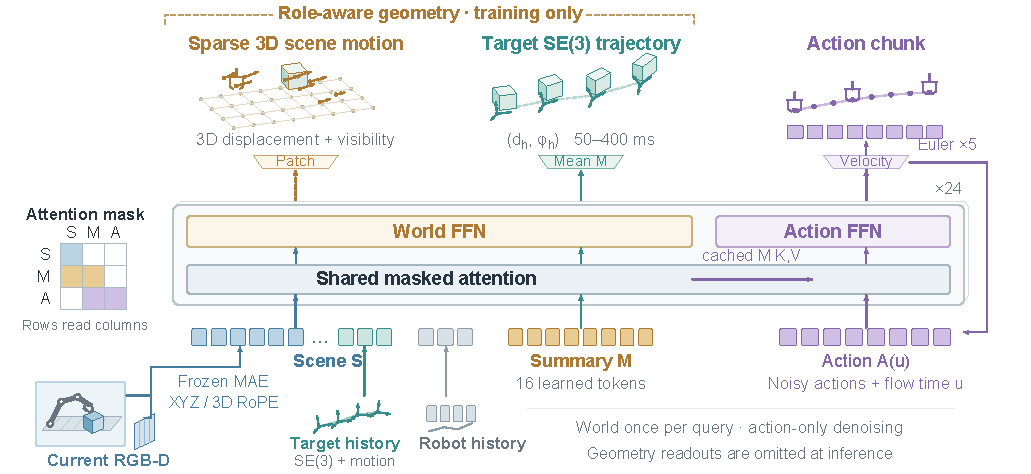
\includegraphics[width=\textwidth]{figures/Fig2/fig2_se3wam.pdf}
\caption{\textbf{\ours 架构。}(a) 自下而上阅读。当前 RGB-D 和目标、机器人状态历史组成场景 token $S$，16 个可学习摘要 token $M$ 补全世界流。12 层主干共享注意力投影，世界流与动作流使用独立的 FFN。仅训练时使用的读出头（虚线）从 patch 状态预测稀疏场景位移和可见性，从摘要均值预测目标 SE(3) 轨迹；辅助监督目标列于几何面板下方。几何示例展示覆盖 50--400\,ms 的 8 个时域中的 3 个实录标签：灰色 glyph 表示当前位姿，橙色 glyph 表示未来位姿（glyph 大小为示意）；当前点云上的位移箭头统一放大 $3\times$。动作图标为示意。(b) 掩码的行表示 query，列表示 key：$S$ 读取 $S$，$M$ 读取 $S,M$，$A$ 读取 $S,M,A$。动作读取世界隐状态。(c) 推理时跳过预测读出头，每次查询只计算并缓存一次世界流的键和值，在 \cfgEuler{} 个 Euler 动作步中复用。}
\label{fig:architecture}
\end{figure*}
